%\section{Architecture and Design}
\section{\dd{} Architecture}
\label{sec:design}

\begin{figure}[t]
  \centering
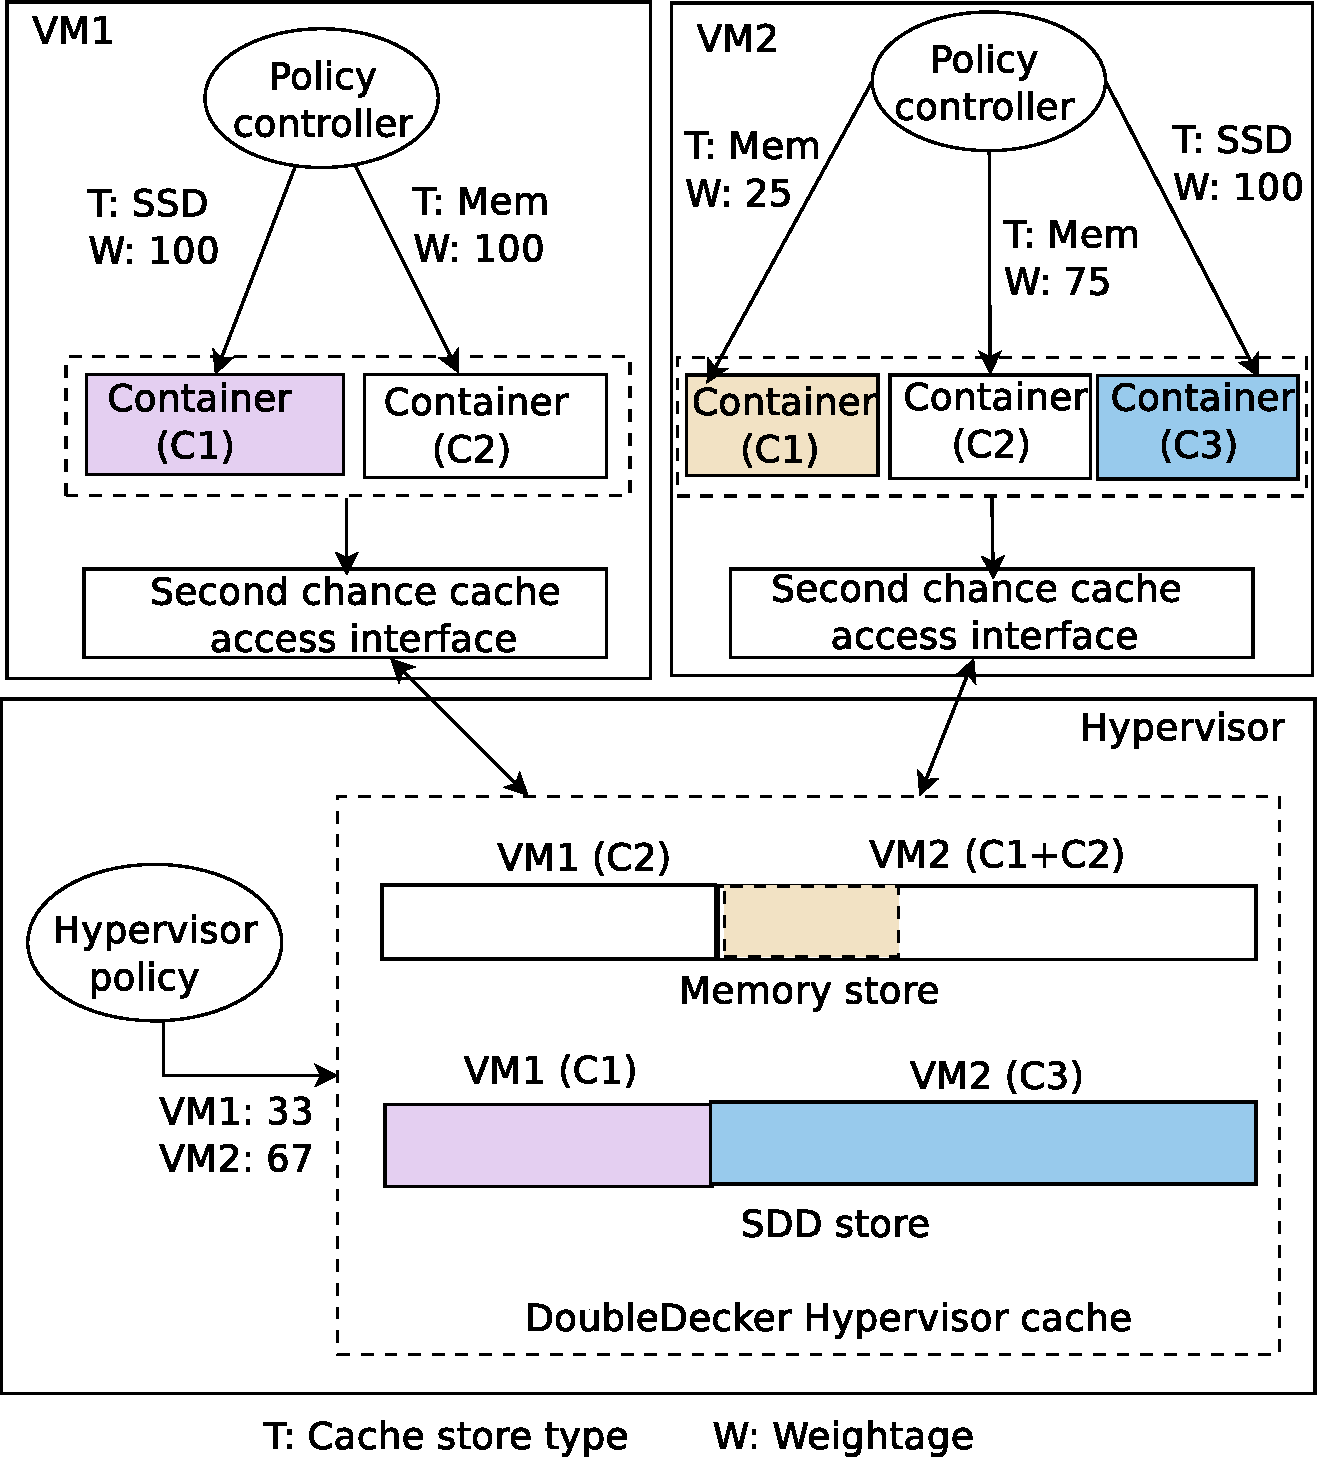
\includegraphics[width=0.42\textwidth]{images/arch} 
 \caption{Proposed differentiated hypervisor cache partitioning 
          across containers in a nested virtualization setting.
	 % \puru{figure needs updates. 1:2 vs. 25:75:100 ... consistently
	 % lets use ratios or weights. Should also probably include a ddecker
	 % cache manager in the hypervisor.}
         }
 \label{fig:desired} 
\vspace{-0.3cm}
\end{figure}

\dd{} provides a 
multi-layered differentiated cache partitioning and management solution.
%\dd{} solution framework for container aware hypervisor caching
%with multi-layered differentiated cache partitioning and management
%is presented in Figure~\ref{fig:desired}.
%
The software architecture of \dd{} is as shown in Figure~\ref{fig:desired}.
Its two main components are the second chance cache interface housed
in each virtual machine and the \dd{} cache manager augmenting the 
hypervisor.
%
The hypervisor cache is managed via two policy controllers,
one to control per-VM provisioning and the other
to control per-container provisioning in the corresponding
virtual machines cache region.
%
Our current design specifies allocations in terms of cache 
usage \revised{weights} in percentage between peer entities at 
each hosting level. 
%
Additionally, the policy controller in each virtual machine
also specifies the cache store type of each container.
%
A two tuple \texttt{<T, W>} is used for this purpose,
where, \texttt{T} denotes the store type (in-memory or SSD)
and \texttt{W} the weight specification for relative sizing.
%
%To configure and manage hypervisor cache, two policy control interfaces provided in 
%the proposed design---(i) VM level policy configuration by the hypervisor, (ii) Container
%level policy specification by the VM administrator. 
%
%The VM level policy is specified in relative weights of the VMs using which
%the hypervisor cache is partitioned across the VMs.  
%%
%Container level policy is specified by a two tuple for each VM---(i) T: cache store type,
%(ii) W: cache usage percentage.
%%
%Cache store type (T) in the proposed architecture is to provide support for multiple types of
%cache stores which can be queried from the VMs and every container can be configured
%with storage backend type as dictated by the policy.
%

Figure~\ref{fig:desired} shows a setup with two virtual machines
with a cache allocation \revised{weight} percentage of 33 and 67. 
The per-VM ratio is
applied to both the memory and the SSD store across all VMs
\footnote{A generalized setup where different cache size
ratios are specified per-VM for the two stores is a straightforward
extension.}.
%
The first virtual machine, VM1 hosts two containers and the second VM (VM2)
hosts three containers.
%In the example setup shown in Figure~\ref{fig:desired}, 
%there are two VMs---VM1 and VM2---configured with weightage
%ratio of 1:2 by the hypervisor.
%
%Two and three application containers are instantiated in VM1 and VM2%,
%respectively.
%
%Each VM administrator can use the policy interface to
%specify the weights for each container's hypervisor cache share.
%
Virtual machine administrators use the local policy controller
to specify distribution of the per-VM cache space across containers.
%
For the example shown, the specification for VM1 for its two
containers is $<$SSD, 100$>$ and $<$Mem, 100$>$---Container 1 to be allotted
all of VM1's share in the SSD store of the hypervisor cache and Container 2
to be allotted all of VM1's share in the memory store of the cache.
%
Similarly, the specification for VM2 is to allocate its memory
store in the ratio of 1:3 for the first two containers and allocate
all of its share in the SSD store to the third container.
%
%In this case, Container 1 and Container 2 of VM1 are configured to use the 
%VM's share of SSD and memory backed cache store, respectively.
%
%
%Container 1 and Container 2 of VM2 are configured with memory backed 
%hypervisor cache with usage percentages as 25 and 75, respectively. 
%
%Container 3 of VM2 is configured to used SSD backed cache store.
%
Based on the above specifications the hypervisor memory store
is shared by three containers and the SSD store by two.
%
Simultaneously, the \revised{weights} for VM1 and VM2 for both the stores
are 33 and 67, respectively.
%
%As shown in the Figure~\ref{fig:desired}, hypervisor cache gets
%distributed depending on the configured weightages at two levels---between
%VMs and across containers within each VM.
%
%Hypervisor memory store is shared by three containers---Container 2 of VM1 and,
%Container 1 and Container 2 of VM2---in the proportions derived by first applying
%relative VM weightage and next by applying container share limits within each VM's
%share.  
%
%Similarly, SSD backed hypervisor cache is shared by Container 1 of VM1 and Container
%3 of VM2 in the ratio of the relative priorities of the VMs.
%
%Different components in the proposed design are explained further.
%\puru{add transition line here.}

\subsection{Policy control mechanism}
The \cgroup{} resource control framework for instantiating containers
provides configuration options to specify allocation limits 
for different resources, e.g.,
CPU share, memory usage limit etc. per-cgroup.
%
Additionally, for each container, the \dd{} policy controller requires 
specification of the hypervisor cache storage type and weight for cache sizing.
%
An extension to the \cgroup{} resource control framework is warranted to 
incorporate this feature.
%
Similar to the dynamic adjustment of resource limits, the hypervisor
cache specifications are required to be handled in dynamic manner.
%the additional configurability related to hypervisor caching.
%
%Container resource control through \cgroups{} should support dynamic
%specification of the policy and propagation of the same to the hypervisor 
%cache store.
%
Interfacing of the updated \cgroup{} resource control framework 
also requires extensions to the second chance cache access 
interface in the guest OS.
%with the hypervisor cache
%interface requires redesign of the hypervisor cache interface.

\subsection{Second chance cache access interface}
The second chance cache interface (explained in \S\ref{sec:bg}) 
assigns unique pool identifiers to each file system registered to use the 
second chance cache by delegating the call to the cache store
implementation.
%
The unique pool identifier is an integral part in the key 
used for operations like lookup, store etc..
%
%which is used for second chance cache operations
%like \get, \put{} and \flush. 
%
%In the proposed system, 
In a derivative cloud setup several containers can be instantiated 
within a single file system, making file system based identifiers 
not applicable.
%which implies file system IDs can not be used as an identification for 
%containers.
%
Towards addressing this, extensions to the \cgroups{} subsystem and 
the second chance cache interface need to be integrated so that 
an unique identity is assigned to each application container 
for use by the hypervisor cache.
%This fundamental change requires redesign of the interface in such 
%a manner that
%each application container uses an unique identity which is assigned 
%by the hypervisor cache store.
%
When an application container boots up, the hypervisor cache interface 
is notified by the \cgroups{} subsystem, which in turn
requests a new pool-ID from the hypervisor cache.
%and assigns the pool ID
%to the application container for its life time.
%
Subsequent second chance cache accesses 
issued by the guest OS are accompanied by the container specific
unique pool identifier.
%because of page cache
%look up failures or evictions 
%
The unique pool-ID is derived by determining the container for the 
operation.
%
%For example, a second chance lookup (\get) request for a file block is first mapped
%to the application container responsible for this lookup to derive the pool ID and pass it 
%on to the hypervisor cache store.
%
%
\subsection{Hypervisor cache store}
%
The cache store implementation of \dd{} %hypervisor cache store 
is required to support container-level policies apart from 
providing VM-level cache partitioning. 
%
The VM-level cache partition sizes are derived from 
ratios specified via the hypervisor-level policy controller.
%\puru{administrator vs. hypervisor level policy.}
%administrator configured ratios 
%
To apply application container level policies, configurations for
containers are transmitted to the hypervisor cache manager
via the guest OS cache interface.
%delegated to the hypervisor cache.
%
%As mentioned earlier, every application container is assigned an unique
%pool ID on start up.
%
The hypervisor cache store applies the policies to partition the
cache across the containers of a virtual machine and also maintains
cache proportionality across virtual machine.
%
The \dd{} solution provides backend storage implementation with
support for dynamic reconfiguration of policies, both at the
hypervisor-level and from within virtual machines. 
%
This feature is required
for dynamic provisioning with changing workload characteristics of
applications and to handle instantiation and removal of virtual
machines and containers.
%
With the derivative setup, a virtual machine can choose to store
objects of all its containers in memory, or on the SSD or 
distributed over both in-memory and SSD storage 
%split storage destinations 
on a per-container basis.
%

\revised{The hypervisor cache also implements an eviction procedure
to flush objects in the cache during memory pressure.
%
%As part of this work, we implement a FIFO policy for
%evictions of objects on memory pressure.
%
}
With two types of storage options available,
a \emph{trickle-down} and \emph{trickle-up} cache is possible---
objects evicted from the second-chance cache are stored
in the third-chance cache.
%
The design of \dd{} is centered around the idea that the
semantics and decisions of how to manage the hypervisor cache
should be left to the policy controller in the guest
operating systems.
%
This offers flexibility to the policy engine to explicitly 
size and choose the storage type for individual applications.
%
For example, a policy engine can decide that an application
that does mostly sequential reads or one whose working set
size is very large, should have its objects stored in 
the SSD.
%
%Storing such objects and then ``spilling'' them over the
%third-chance cache will only pollute the second-chance
%cache.
%
%We present empirical results to demonstrate this in Section~\ref{sec:expt}.
Nevertheless, keeping the core principle of supporting cache management from 
within the VM, we provide a hybrid mode configuration option for the
VM-level controller.
%
In this mode, the VM-level controller can provision containers 
with both memory and SSD shares, where the SSD store is used only when the
memory share of the container is exhausted. 
%
The comprehensive design and evaluation of the hybrid store
is left as a future direction. 
%
In this work, we present
results with applications configured to use either in-memory
or SSD backed caches, not both.
%
%
%memory and SSD.
%
%Depending on memory type configuration for the containers, the requests
%are stored either in the memory store or the SSD store.
%

\revised{
While exclusive caching takes care of deduplication of memory across 
the hypervisor cache and page cache of individual virtual machines, there is 
a chance of content duplication across virtual machines and the hypervisor
cache.
%
Holistic deduplication techniques in virtualized systems~\cite{synergy} can be 
incorporated into DoubleDecker to address the issue of duplication and left as
a future direction. 
}
